\documentclass[1p]{elsarticle_modified}
%\bibliographystyle{elsarticle-num}

%\usepackage[colorlinks]{hyperref}
%\usepackage{abbrmath_seonhwa} %\Abb, \Ascr, \Acal ,\Abf, \Afrak
\usepackage{amsfonts}
\usepackage{amssymb}
\usepackage{amsmath}
\usepackage{amsthm}
\usepackage{scalefnt}
\usepackage{amsbsy}
\usepackage{kotex}
\usepackage{caption}
\usepackage{subfig}
\usepackage{color}
\usepackage{graphicx}
\usepackage{xcolor} %% white, black, red, green, blue, cyan, magenta, yellow
\usepackage{float}
\usepackage{setspace}
\usepackage{hyperref}

\usepackage{tikz}
\usetikzlibrary{arrows}

\usepackage{multirow}
\usepackage{array} % fixed length table
\usepackage{hhline}

%%%%%%%%%%%%%%%%%%%%%
\makeatletter
\renewcommand*\env@matrix[1][\arraystretch]{%
	\edef\arraystretch{#1}%
	\hskip -\arraycolsep
	\let\@ifnextchar\new@ifnextchar
	\array{*\c@MaxMatrixCols c}}
\makeatother %https://tex.stackexchange.com/questions/14071/how-can-i-increase-the-line-spacing-in-a-matrix
%%%%%%%%%%%%%%%

\usepackage[normalem]{ulem}

\newcommand{\msout}[1]{\ifmmode\text{\sout{\ensuremath{#1}}}\else\sout{#1}\fi}
%SOURCE: \msout is \stkout macro in https://tex.stackexchange.com/questions/20609/strikeout-in-math-mode

\newcommand{\cancel}[1]{
	\ifmmode
	{\color{red}\msout{#1}}
	\else
	{\color{red}\sout{#1}}
	\fi
}

\newcommand{\add}[1]{
	{\color{blue}\uwave{#1}}
}

\newcommand{\replace}[2]{
	\ifmmode
	{\color{red}\msout{#1}}{\color{blue}\uwave{#2}}
	\else
	{\color{red}\sout{#1}}{\color{blue}\uwave{#2}}
	\fi
}

\newcommand{\Sol}{\mathcal{S}} %segment
\newcommand{\D}{D} %diagram
\newcommand{\A}{\mathcal{A}} %arc


%%%%%%%%%%%%%%%%%%%%%%%%%%%%%5 test

\def\sl{\operatorname{\textup{SL}}(2,\Cbb)}
\def\psl{\operatorname{\textup{PSL}}(2,\Cbb)}
\def\quan{\mkern 1mu \triangleright \mkern 1mu}

\theoremstyle{definition}
\newtheorem{thm}{Theorem}[section]
\newtheorem{prop}[thm]{Proposition}
\newtheorem{lem}[thm]{Lemma}
\newtheorem{ques}[thm]{Question}
\newtheorem{cor}[thm]{Corollary}
\newtheorem{defn}[thm]{Definition}
\newtheorem{exam}[thm]{Example}
\newtheorem{rmk}[thm]{Remark}
\newtheorem{alg}[thm]{Algorithm}

\newcommand{\I}{\sqrt{-1}}
\begin{document}

%\begin{frontmatter}
%
%\title{Boundary parabolic representations of knots up to 8 crossings}
%
%%% Group authors per affiliation:
%\author{Yunhi Cho} 
%\address{Department of Mathematics, University of Seoul, Seoul, Korea}
%\ead{yhcho@uos.ac.kr}
%
%
%\author{Seonhwa Kim} %\fnref{s_kim}}
%\address{Center for Geometry and Physics, Institute for Basic Science, Pohang, 37673, Korea}
%\ead{ryeona17@ibs.re.kr}
%
%\author{Hyuk Kim}
%\address{Department of Mathematical Sciences, Seoul National University, Seoul 08826, Korea}
%\ead{hyukkim@snu.ac.kr}
%
%\author{Seokbeom Yoon}
%\address{Department of Mathematical Sciences, Seoul National University, Seoul, 08826,  Korea}
%\ead{sbyoon15@snu.ac.kr}
%
%\begin{abstract}
%We find all boundary parabolic representation of knots up to 8 crossings.
%
%\end{abstract}
%\begin{keyword}
%    \MSC[2010] 57M25 
%\end{keyword}
%
%\end{frontmatter}

%\linenumbers
%\tableofcontents
%
\newcommand\colored[1]{\textcolor{white}{\rule[-0.35ex]{0.8em}{1.4ex}}\kern-0.8em\color{red} #1}%
%\newcommand\colored[1]{\textcolor{white}{ #1}\kern-2.17ex	\textcolor{white}{ #1}\kern-1.81ex	\textcolor{white}{ #1}\kern-2.15ex\color{red}#1	}

{\Large $\underline{12a_{0663}~(K12a_{0663})}$}

\setlength{\tabcolsep}{10pt}
\renewcommand{\arraystretch}{1.6}
\vspace{1cm}\begin{tabular}{m{100pt}>{\centering\arraybackslash}m{274pt}}
\multirow{5}{120pt}{
	\centering
	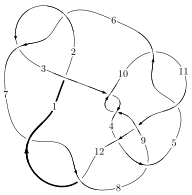
\includegraphics[width=112pt]{../../../GIT/diagram.site/Diagrams/png/1464_12a_0663.png}\\
\ \ \ A knot diagram\footnotemark}&
\allowdisplaybreaks
\textbf{Linearized knot diagam} \\
\cline{2-2}
 &
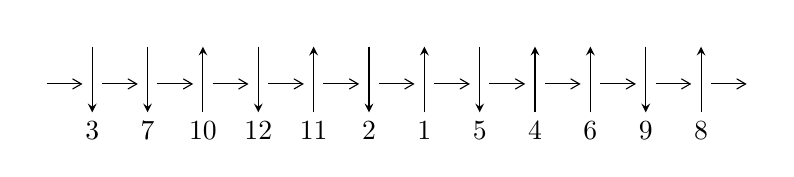
\begin{tikzpicture}[x=20pt, y=17pt]
	% nodes
	\node (C0) at (0, 0) {};
	\node (C1) at (1, 0) {};
	\node (C1U) at (1, +1) {};
	\node (C1D) at (1, -1) {3};

	\node (C2) at (2, 0) {};
	\node (C2U) at (2, +1) {};
	\node (C2D) at (2, -1) {7};

	\node (C3) at (3, 0) {};
	\node (C3U) at (3, +1) {};
	\node (C3D) at (3, -1) {10};

	\node (C4) at (4, 0) {};
	\node (C4U) at (4, +1) {};
	\node (C4D) at (4, -1) {12};

	\node (C5) at (5, 0) {};
	\node (C5U) at (5, +1) {};
	\node (C5D) at (5, -1) {11};

	\node (C6) at (6, 0) {};
	\node (C6U) at (6, +1) {};
	\node (C6D) at (6, -1) {2};

	\node (C7) at (7, 0) {};
	\node (C7U) at (7, +1) {};
	\node (C7D) at (7, -1) {1};

	\node (C8) at (8, 0) {};
	\node (C8U) at (8, +1) {};
	\node (C8D) at (8, -1) {5};

	\node (C9) at (9, 0) {};
	\node (C9U) at (9, +1) {};
	\node (C9D) at (9, -1) {4};

	\node (C10) at (10, 0) {};
	\node (C10U) at (10, +1) {};
	\node (C10D) at (10, -1) {6};

	\node (C11) at (11, 0) {};
	\node (C11U) at (11, +1) {};
	\node (C11D) at (11, -1) {9};

	\node (C12) at (12, 0) {};
	\node (C12U) at (12, +1) {};
	\node (C12D) at (12, -1) {8};
	\node (C13) at (13, 0) {};

	% arrows
	\draw[->,>={angle 60}]
	(C0) edge (C1) (C1) edge (C2) (C2) edge (C3) (C3) edge (C4) (C4) edge (C5) (C5) edge (C6) (C6) edge (C7) (C7) edge (C8) (C8) edge (C9) (C9) edge (C10) (C10) edge (C11) (C11) edge (C12) (C12) edge (C13) ;	\draw[->,>=stealth]
	(C1U) edge (C1D) (C2U) edge (C2D) (C3D) edge (C3U) (C4U) edge (C4D) (C5D) edge (C5U) (C6U) edge (C6D) (C7D) edge (C7U) (C8U) edge (C8D) (C9D) edge (C9U) (C10D) edge (C10U) (C11U) edge (C11D) (C12D) edge (C12U) ;
	\end{tikzpicture} \\
\hhline{~~} \\& 
\textbf{Solving Sequence} \\ \cline{2-2} 
 &
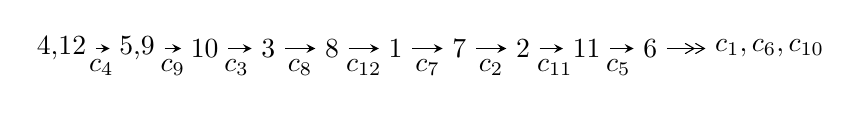
\begin{tikzpicture}[x=23pt, y=7pt]
	% node
	\node (A0) at (-1/8, 0) {4,12};
	\node (A1) at (17/16, 0) {5,9};
	\node (A2) at (17/8, 0) {10};
	\node (A3) at (25/8, 0) {3};
	\node (A4) at (33/8, 0) {8};
	\node (A5) at (41/8, 0) {1};
	\node (A6) at (49/8, 0) {7};
	\node (A7) at (57/8, 0) {2};
	\node (A8) at (65/8, 0) {11};
	\node (A9) at (73/8, 0) {6};
	\node (C1) at (1/2, -1) {$c_{4}$};
	\node (C2) at (13/8, -1) {$c_{9}$};
	\node (C3) at (21/8, -1) {$c_{3}$};
	\node (C4) at (29/8, -1) {$c_{8}$};
	\node (C5) at (37/8, -1) {$c_{12}$};
	\node (C6) at (45/8, -1) {$c_{7}$};
	\node (C7) at (53/8, -1) {$c_{2}$};
	\node (C8) at (61/8, -1) {$c_{11}$};
	\node (C9) at (69/8, -1) {$c_{5}$};
	\node (A10) at (11, 0) {$c_{1},c_{6},c_{10}$};

	% edge
	\draw[->,>=stealth]	
	(A0) edge (A1) (A1) edge (A2) (A2) edge (A3) (A3) edge (A4) (A4) edge (A5) (A5) edge (A6) (A6) edge (A7) (A7) edge (A8) (A8) edge (A9) ;
	\draw[->>,>={angle 60}]	
	(A9) edge (A10);
\end{tikzpicture} \\ 

\end{tabular} \\

\footnotetext{
The image of knot diagram is generated by the software ``\textbf{Draw programme}" developed by Andrew Bartholomew(\url{http://www.layer8.co.uk/maths/draw/index.htm\#Running-draw}), where we modified some parts for our purpose(\url{https://github.com/CATsTAILs/LinksPainter}).
}\phantom \\ \newline 
\centering \textbf{Ideals for irreducible components\footnotemark of $X_{\text{par}}$} 
 
\begin{align*}
I^u_{1}&=\langle 
-6.53926\times10^{31} u^{38}-4.08337\times10^{30} u^{37}+\cdots+6.57846\times10^{31} b+8.43133\times10^{30},\\
\phantom{I^u_{1}}&\phantom{= \langle  }-1.38800\times10^{31} u^{38}-2.23113\times10^{31} u^{37}+\cdots+6.57846\times10^{31} a-3.08771\times10^{32},\;u^{39}+u^{38}+\cdots+7 u^2+1\rangle \\
I^u_{2}&=\langle 
-6.98995\times10^{294} u^{71}-1.49499\times10^{295} u^{70}+\cdots+1.56256\times10^{295} b-1.00003\times10^{298},\\
\phantom{I^u_{2}}&\phantom{= \langle  }-4.22283\times10^{228} u^{71}-9.43208\times10^{228} u^{70}+\cdots+1.97531\times10^{229} a-7.72233\times10^{231},\\
\phantom{I^u_{2}}&\phantom{= \langle  }u^{72}+3 u^{71}+\cdots-300 u+1393\rangle \\
I^u_{3}&=\langle 
-227849189 u^{23}-908034262 u^{22}+\cdots+2211913739 b-16196133,\\
\phantom{I^u_{3}}&\phantom{= \langle  }18343895 u^{23}-2147762 u^{22}+\cdots+2211913739 a+1387418052,\;u^{24}- u^{23}+\cdots-2 u+1\rangle \\
\\
\end{align*}
\raggedright * 3 irreducible components of $\dim_{\mathbb{C}}=0$, with total 135 representations.\\
\footnotetext{All coefficients of polynomials are rational numbers. But the coefficients are sometimes approximated in decimal forms when there is not enough margin.}
\newpage
\renewcommand{\arraystretch}{1}
\centering \section*{I. $I^u_{1}= \langle -6.54\times10^{31} u^{38}-4.08\times10^{30} u^{37}+\cdots+6.58\times10^{31} b+8.43\times10^{30},\;-1.39\times10^{31} u^{38}-2.23\times10^{31} u^{37}+\cdots+6.58\times10^{31} a-3.09\times10^{32},\;u^{39}+u^{38}+\cdots+7 u^2+1 \rangle$}
\flushleft \textbf{(i) Arc colorings}\\
\begin{tabular}{m{7pt} m{180pt} m{7pt} m{180pt} }
\flushright $a_{4}=$&$\begin{pmatrix}1\\0\end{pmatrix}$ \\
\flushright $a_{12}=$&$\begin{pmatrix}0\\u\end{pmatrix}$ \\
\flushright $a_{5}=$&$\begin{pmatrix}1\\u^2\end{pmatrix}$ \\
\flushright $a_{9}=$&$\begin{pmatrix}0.210991 u^{38}+0.339157 u^{37}+\cdots-4.36758 u+4.69367\\0.994042 u^{38}+0.0620718 u^{37}+\cdots+0.789009 u-0.128166\end{pmatrix}$ \\
\flushright $a_{10}=$&$\begin{pmatrix}1.20503 u^{38}+0.401229 u^{37}+\cdots-3.57857 u+4.56550\\0.994042 u^{38}+0.0620718 u^{37}+\cdots+0.789009 u-0.128166\end{pmatrix}$ \\
\flushright $a_{3}=$&$\begin{pmatrix}5.20733 u^{38}+1.32756 u^{37}+\cdots-1.16737 u+6.24635\\1.20174 u^{38}-0.260291 u^{37}+\cdots-4.13375 u+1.42369\end{pmatrix}$ \\
\flushright $a_{8}=$&$\begin{pmatrix}0.210991 u^{38}+0.339157 u^{37}+\cdots-3.36758 u+4.69367\\0.994042 u^{38}+0.0620718 u^{37}+\cdots+0.789009 u-0.128166\end{pmatrix}$ \\
\flushright $a_{1}=$&$\begin{pmatrix}-2.04556 u^{38}-0.0320806 u^{37}+\cdots+6.93865 u-1.98362\\-0.970929 u^{38}-0.311046 u^{37}+\cdots+2.83457 u-2.14165\end{pmatrix}$ \\
\flushright $a_{7}=$&$\begin{pmatrix}1.03526 u^{38}+0.698475 u^{37}+\cdots+0.632919 u+5.82032\\-0.0773108 u^{38}-0.183940 u^{37}+\cdots+1.79931 u-1.80486\end{pmatrix}$ \\
\flushright $a_{2}=$&$\begin{pmatrix}0.410708 u^{38}+0.579404 u^{37}+\cdots+4.25907 u+3.42658\\-1.55656 u^{38}-0.282778 u^{37}+\cdots+2.55983 u-2.67790\end{pmatrix}$ \\
\flushright $a_{11}=$&$\begin{pmatrix}-4.03365 u^{38}-0.156224 u^{37}+\cdots+7.36063 u-1.72729\\-2.41774 u^{38}-0.284021 u^{37}+\cdots+4.82266 u-4.00559\end{pmatrix}$ \\
\flushright $a_{6}=$&$\begin{pmatrix}3.57384 u^{38}+0.937443 u^{37}+\cdots-8.23572 u+5.85575\\1.32991 u^{38}+0.861916 u^{37}+\cdots+0.559915 u+1.21270\end{pmatrix}$\\&\end{tabular}
\flushleft \textbf{(ii) Obstruction class $= -1$}\\~\\
\flushleft \textbf{(iii) Cusp Shapes $= 9.50767 u^{38}+2.94061 u^{37}+\cdots-7.93931 u-0.143921$}\\~\\
\newpage\renewcommand{\arraystretch}{1}
\flushleft \textbf{(iv) u-Polynomials at the component}\newline \\
\begin{tabular}{m{50pt}|m{274pt}}
Crossings & \hspace{64pt}u-Polynomials at each crossing \\
\hline $$\begin{aligned}c_{1}\end{aligned}$$&$\begin{aligned}
&u^{39}+21 u^{38}+\cdots+16 u+64
\end{aligned}$\\
\hline $$\begin{aligned}c_{2},c_{6}\end{aligned}$$&$\begin{aligned}
&u^{39}-7 u^{38}+\cdots-68 u+8
\end{aligned}$\\
\hline $$\begin{aligned}c_{3},c_{5},c_{9}\\c_{10}\end{aligned}$$&$\begin{aligned}
&u^{39}+20 u^{37}+\cdots- u+1
\end{aligned}$\\
\hline $$\begin{aligned}c_{4},c_{8}\end{aligned}$$&$\begin{aligned}
&u^{39}+u^{38}+\cdots+7 u^2+1
\end{aligned}$\\
\hline $$\begin{aligned}c_{7},c_{12}\end{aligned}$$&$\begin{aligned}
&u^{39}-21 u^{38}+\cdots-10052 u+1192
\end{aligned}$\\
\hline $$\begin{aligned}c_{11}\end{aligned}$$&$\begin{aligned}
&u^{39}-36 u^{38}+\cdots+90112 u-4096
\end{aligned}$\\
\hline
\end{tabular}\\~\\
\newpage\renewcommand{\arraystretch}{1}
\flushleft \textbf{(v) Riley Polynomials at the component}\newline \\
\begin{tabular}{m{50pt}|m{274pt}}
Crossings & \hspace{64pt}Riley Polynomials at each crossing \\
\hline $$\begin{aligned}c_{1}\end{aligned}$$&$\begin{aligned}
&y^{39}-5 y^{38}+\cdots-2816 y-4096
\end{aligned}$\\
\hline $$\begin{aligned}c_{2},c_{6}\end{aligned}$$&$\begin{aligned}
&y^{39}-21 y^{38}+\cdots+16 y-64
\end{aligned}$\\
\hline $$\begin{aligned}c_{3},c_{5},c_{9}\\c_{10}\end{aligned}$$&$\begin{aligned}
&y^{39}+40 y^{38}+\cdots+19 y-1
\end{aligned}$\\
\hline $$\begin{aligned}c_{4},c_{8}\end{aligned}$$&$\begin{aligned}
&y^{39}-15 y^{38}+\cdots-14 y-1
\end{aligned}$\\
\hline $$\begin{aligned}c_{7},c_{12}\end{aligned}$$&$\begin{aligned}
&y^{39}+31 y^{38}+\cdots+64653328 y-1420864
\end{aligned}$\\
\hline $$\begin{aligned}c_{11}\end{aligned}$$&$\begin{aligned}
&y^{39}-10 y^{38}+\cdots+125829120 y-16777216
\end{aligned}$\\
\hline
\end{tabular}\\~\\
\newpage\flushleft \textbf{(vi) Complex Volumes and Cusp Shapes}
$$\begin{array}{c|c|c}  
\text{Solutions to }I^u_{1}& \I (\text{vol} + \sqrt{-1}CS) & \text{Cusp shape}\\
 \hline 
\begin{aligned}
u &= -0.567111 + 0.787760 I \\
a &= \phantom{-}0.697115 + 0.159087 I \\
b &= -0.633371 + 0.117333 I\end{aligned}
 & \phantom{-}1.32490 + 3.31400 I & \phantom{-}4.45912 - 5.74087 I \\ \hline\begin{aligned}
u &= -0.567111 - 0.787760 I \\
a &= \phantom{-}0.697115 - 0.159087 I \\
b &= -0.633371 - 0.117333 I\end{aligned}
 & \phantom{-}1.32490 - 3.31400 I & \phantom{-}4.45912 + 5.74087 I \\ \hline\begin{aligned}
u &= -0.765136 + 0.571280 I \\
a &= \phantom{-}2.16539 + 0.12213 I \\
b &= -0.097378 - 1.290100 I\end{aligned}
 & -4.07768 + 4.05588 I & -5.30316 - 7.20111 I \\ \hline\begin{aligned}
u &= -0.765136 - 0.571280 I \\
a &= \phantom{-}2.16539 - 0.12213 I \\
b &= -0.097378 + 1.290100 I\end{aligned}
 & -4.07768 - 4.05588 I & -5.30316 + 7.20111 I \\ \hline\begin{aligned}
u &= -0.943048 + 0.012408 I \\
a &= \phantom{-}1.34635 - 1.58586 I \\
b &= \phantom{-}0.21700 - 1.42922 I\end{aligned}
 & -15.0496 + 1.0975 I & -12.20549 - 0.94590 I \\ \hline\begin{aligned}
u &= -0.943048 - 0.012408 I \\
a &= \phantom{-}1.34635 + 1.58586 I \\
b &= \phantom{-}0.21700 + 1.42922 I\end{aligned}
 & -15.0496 - 1.0975 I & -12.20549 + 0.94590 I \\ \hline\begin{aligned}
u &= -0.852570 + 0.138373 I \\
a &= \phantom{-}0.96600 + 2.04699 I \\
b &= \phantom{-}0.314074 + 1.359160 I\end{aligned}
 & -13.8330 + 8.7861 I & -10.86252 - 6.43696 I \\ \hline\begin{aligned}
u &= -0.852570 - 0.138373 I \\
a &= \phantom{-}0.96600 - 2.04699 I \\
b &= \phantom{-}0.314074 - 1.359160 I\end{aligned}
 & -13.8330 - 8.7861 I & -10.86252 + 6.43696 I \\ \hline\begin{aligned}
u &= \phantom{-}0.837375 + 0.048442 I \\
a &= -1.32421 + 2.02490 I \\
b &= -0.252328 + 1.356110 I\end{aligned}
 & -10.43840 - 3.43951 I & -9.01036 + 2.72933 I \\ \hline\begin{aligned}
u &= \phantom{-}0.837375 - 0.048442 I \\
a &= -1.32421 - 2.02490 I \\
b &= -0.252328 - 1.356110 I\end{aligned}
 & -10.43840 + 3.43951 I & -9.01036 - 2.72933 I\\
 \hline 
 \end{array}$$\newpage$$\begin{array}{c|c|c}  
\text{Solutions to }I^u_{1}& \I (\text{vol} + \sqrt{-1}CS) & \text{Cusp shape}\\
 \hline 
\begin{aligned}
u &= \phantom{-}0.695786 + 0.401836 I \\
a &= -2.78898 - 0.37450 I \\
b &= \phantom{-}0.005349 - 1.278550 I\end{aligned}
 & -4.95357 + 1.37371 I & -9.10851 + 2.59492 I \\ \hline\begin{aligned}
u &= \phantom{-}0.695786 - 0.401836 I \\
a &= -2.78898 + 0.37450 I \\
b &= \phantom{-}0.005349 + 1.278550 I\end{aligned}
 & -4.95357 - 1.37371 I & -9.10851 - 2.59492 I \\ \hline\begin{aligned}
u &= \phantom{-}0.351727 + 0.722046 I \\
a &= -0.822254 + 0.137329 I \\
b &= \phantom{-}0.608935 + 0.249794 I\end{aligned}
 & \phantom{-}1.85851 + 0.64123 I & \phantom{-}6.33062 - 2.65229 I \\ \hline\begin{aligned}
u &= \phantom{-}0.351727 - 0.722046 I \\
a &= -0.822254 - 0.137329 I \\
b &= \phantom{-}0.608935 - 0.249794 I\end{aligned}
 & \phantom{-}1.85851 - 0.64123 I & \phantom{-}6.33062 + 2.65229 I \\ \hline\begin{aligned}
u &= -0.967742 + 0.763288 I \\
a &= \phantom{-}0.568572 + 0.141085 I \\
b &= -0.558086 - 0.026749 I\end{aligned}
 & -1.51812 + 3.17788 I & \phantom{-}2.76285 - 2.10152 I \\ \hline\begin{aligned}
u &= -0.967742 - 0.763288 I \\
a &= \phantom{-}0.568572 - 0.141085 I \\
b &= -0.558086 + 0.026749 I\end{aligned}
 & -1.51812 - 3.17788 I & \phantom{-}2.76285 + 2.10152 I \\ \hline\begin{aligned}
u &= \phantom{-}1.082180 + 0.592049 I \\
a &= -1.46368 - 0.22780 I \\
b &= \phantom{-}0.17300 - 1.47046 I\end{aligned}
 & -10.66960 - 5.07856 I & -10.53992 + 4.00671 I \\ \hline\begin{aligned}
u &= \phantom{-}1.082180 - 0.592049 I \\
a &= -1.46368 + 0.22780 I \\
b &= \phantom{-}0.17300 + 1.47046 I\end{aligned}
 & -10.66960 + 5.07856 I & -10.53992 - 4.00671 I \\ \hline\begin{aligned}
u &= -0.764518\phantom{ +0.000000I} \\
a &= \phantom{-}0.569386\phantom{ +0.000000I} \\
b &= -0.431719\phantom{ +0.000000I}\end{aligned}
 & -1.66339\phantom{ +0.000000I} & -4.64910\phantom{ +0.000000I} \\ \hline\begin{aligned}
u &= \phantom{-}1.093730 + 0.671358 I \\
a &= -0.540699 + 0.117342 I \\
b &= \phantom{-}0.518302 - 0.035214 I\end{aligned}
 & -5.30148 + 0.79401 I & -2.08945 - 2.40704 I\\
 \hline 
 \end{array}$$\newpage$$\begin{array}{c|c|c}  
\text{Solutions to }I^u_{1}& \I (\text{vol} + \sqrt{-1}CS) & \text{Cusp shape}\\
 \hline 
\begin{aligned}
u &= \phantom{-}1.093730 - 0.671358 I \\
a &= -0.540699 - 0.117342 I \\
b &= \phantom{-}0.518302 + 0.035214 I\end{aligned}
 & -5.30148 - 0.79401 I & -2.08945 + 2.40704 I \\ \hline\begin{aligned}
u &= -0.993018 + 0.816568 I \\
a &= \phantom{-}1.369400 + 0.161395 I \\
b &= -0.294026 - 1.352700 I\end{aligned}
 & -4.89712 + 7.00444 I & -3.44470 - 5.09853 I \\ \hline\begin{aligned}
u &= -0.993018 - 0.816568 I \\
a &= \phantom{-}1.369400 - 0.161395 I \\
b &= -0.294026 + 1.352700 I\end{aligned}
 & -4.89712 - 7.00444 I & -3.44470 + 5.09853 I \\ \hline\begin{aligned}
u &= \phantom{-}1.027790 + 0.860017 I \\
a &= -0.550444 + 0.162872 I \\
b &= \phantom{-}0.565522 - 0.061491 I\end{aligned}
 & -4.63847 - 7.81620 I & \phantom{-0.000000 -}0. + 5.15619 I \\ \hline\begin{aligned}
u &= \phantom{-}1.027790 - 0.860017 I \\
a &= -0.550444 - 0.162872 I \\
b &= \phantom{-}0.565522 + 0.061491 I\end{aligned}
 & -4.63847 + 7.81620 I & \phantom{-0.000000 } 0. - 5.15619 I \\ \hline\begin{aligned}
u &= \phantom{-}0.075508 + 0.610308 I \\
a &= \phantom{-}1.53525 + 0.35499 I \\
b &= -0.520301 + 0.621604 I\end{aligned}
 & -1.47213 - 5.06690 I & -0.37269 + 8.17616 I \\ \hline\begin{aligned}
u &= \phantom{-}0.075508 - 0.610308 I \\
a &= \phantom{-}1.53525 - 0.35499 I \\
b &= -0.520301 - 0.621604 I\end{aligned}
 & -1.47213 + 5.06690 I & -0.37269 - 8.17616 I \\ \hline\begin{aligned}
u &= \phantom{-}1.082800 + 0.904573 I \\
a &= -1.192250 + 0.140890 I \\
b &= \phantom{-}0.38451 - 1.38106 I\end{aligned}
 & -6.47260 - 12.07610 I & \phantom{-0.000000 } 0 \\ \hline\begin{aligned}
u &= \phantom{-}1.082800 - 0.904573 I \\
a &= -1.192250 - 0.140890 I \\
b &= \phantom{-}0.38451 + 1.38106 I\end{aligned}
 & -6.47260 + 12.07610 I & \phantom{-0.000000 } 0 \\ \hline\begin{aligned}
u &= \phantom{-}0.093806 + 0.574754 I \\
a &= -1.190660 - 0.013225 I \\
b &= \phantom{-}0.478079 + 0.450617 I\end{aligned}
 & \phantom{-}0.88043 + 1.10691 I & \phantom{-}4.57256 - 4.10450 I\\
 \hline 
 \end{array}$$\newpage$$\begin{array}{c|c|c}  
\text{Solutions to }I^u_{1}& \I (\text{vol} + \sqrt{-1}CS) & \text{Cusp shape}\\
 \hline 
\begin{aligned}
u &= \phantom{-}0.093806 - 0.574754 I \\
a &= -1.190660 + 0.013225 I \\
b &= \phantom{-}0.478079 - 0.450617 I\end{aligned}
 & \phantom{-}0.88043 - 1.10691 I & \phantom{-}4.57256 + 4.10450 I \\ \hline\begin{aligned}
u &= \phantom{-}0.032561 + 0.358979 I \\
a &= \phantom{-}1.98747 - 1.70278 I \\
b &= -0.181643 + 0.623066 I\end{aligned}
 & -1.79359 + 1.44290 I & -3.00301 - 2.32178 I \\ \hline\begin{aligned}
u &= \phantom{-}0.032561 - 0.358979 I \\
a &= \phantom{-}1.98747 + 1.70278 I \\
b &= -0.181643 - 0.623066 I\end{aligned}
 & -1.79359 - 1.44290 I & -3.00301 + 2.32178 I \\ \hline\begin{aligned}
u &= -1.37493 + 0.89777 I \\
a &= \phantom{-}0.985563 - 0.068694 I \\
b &= -0.47573 - 1.60982 I\end{aligned}
 & -16.4040 + 8.0432 I & \phantom{-0.000000 } 0 \\ \hline\begin{aligned}
u &= -1.37493 - 0.89777 I \\
a &= \phantom{-}0.985563 + 0.068694 I \\
b &= -0.47573 + 1.60982 I\end{aligned}
 & -16.4040 - 8.0432 I & \phantom{-0.000000 } 0 \\ \hline\begin{aligned}
u &= \phantom{-}1.34788 + 0.94806 I \\
a &= -0.977771 - 0.023278 I \\
b &= \phantom{-}0.50981 - 1.57225 I\end{aligned}
 & -12.0675 - 12.5408 I & \phantom{-0.000000 } 0 \\ \hline\begin{aligned}
u &= \phantom{-}1.34788 - 0.94806 I \\
a &= -0.977771 + 0.023278 I \\
b &= \phantom{-}0.50981 + 1.57225 I\end{aligned}
 & -12.0675 + 12.5408 I & \phantom{-0.000000 } 0 \\ \hline\begin{aligned}
u &= -1.37533 + 0.98042 I \\
a &= \phantom{-}0.945129 - 0.018463 I \\
b &= -0.54586 - 1.58560 I\end{aligned}
 & -15.4829 + 17.6772 I & \phantom{-0.000000 } 0 \\ \hline\begin{aligned}
u &= -1.37533 - 0.98042 I \\
a &= \phantom{-}0.945129 + 0.018463 I \\
b &= -0.54586 + 1.58560 I\end{aligned}
 & -15.4829 - 17.6772 I & \phantom{-0.000000 } 0\\
 \hline 
 \end{array}$$\newpage\newpage\renewcommand{\arraystretch}{1}
\centering \section*{II. $I^u_{2}= \langle -6.99\times10^{294} u^{71}-1.49\times10^{295} u^{70}+\cdots+1.56\times10^{295} b-1.00\times10^{298},\;-4.22\times10^{228} u^{71}-9.43\times10^{228} u^{70}+\cdots+1.98\times10^{229} a-7.72\times10^{231},\;u^{72}+3 u^{71}+\cdots-300 u+1393 \rangle$}
\flushleft \textbf{(i) Arc colorings}\\
\begin{tabular}{m{7pt} m{180pt} m{7pt} m{180pt} }
\flushright $a_{4}=$&$\begin{pmatrix}1\\0\end{pmatrix}$ \\
\flushright $a_{12}=$&$\begin{pmatrix}0\\u\end{pmatrix}$ \\
\flushright $a_{5}=$&$\begin{pmatrix}1\\u^2\end{pmatrix}$ \\
\flushright $a_{9}=$&$\begin{pmatrix}0.213781 u^{71}+0.477499 u^{70}+\cdots-559.380 u+390.943\\0.447340 u^{71}+0.956757 u^{70}+\cdots-863.774 u+639.995\end{pmatrix}$ \\
\flushright $a_{10}=$&$\begin{pmatrix}0.661121 u^{71}+1.43426 u^{70}+\cdots-1423.15 u+1030.94\\0.447340 u^{71}+0.956757 u^{70}+\cdots-863.774 u+639.995\end{pmatrix}$ \\
\flushright $a_{3}=$&$\begin{pmatrix}-0.326580 u^{71}-0.679236 u^{70}+\cdots+636.636 u-521.167\\-0.652852 u^{71}-1.39754 u^{70}+\cdots+1534.59 u-1128.73\end{pmatrix}$ \\
\flushright $a_{8}=$&$\begin{pmatrix}0.547431 u^{71}+1.17282 u^{70}+\cdots-1076.20 u+802.706\\0.756568 u^{71}+1.61079 u^{70}+\cdots-1420.24 u+1065.74\end{pmatrix}$ \\
\flushright $a_{1}=$&$\begin{pmatrix}0.321622 u^{71}+0.694407 u^{70}+\cdots-667.373 u+482.233\\0.838420 u^{71}+1.84757 u^{70}+\cdots-2017.81 u+1381.44\end{pmatrix}$ \\
\flushright $a_{7}=$&$\begin{pmatrix}-0.712040 u^{71}-1.48815 u^{70}+\cdots+1236.05 u-996.432\\-0.302736 u^{71}-0.544396 u^{70}+\cdots-34.3875 u-183.143\end{pmatrix}$ \\
\flushright $a_{2}=$&$\begin{pmatrix}-1.12512 u^{71}-2.32951 u^{70}+\cdots+1885.56 u-1615.02\\-0.379009 u^{71}-0.633666 u^{70}+\cdots-279.657 u-203.153\end{pmatrix}$ \\
\flushright $a_{11}=$&$\begin{pmatrix}0.0534466 u^{71}+0.0989686 u^{70}+\cdots+24.9761 u+17.5353\\-0.260512 u^{71}-0.587739 u^{70}+\cdots+705.445 u-454.496\end{pmatrix}$ \\
\flushright $a_{6}=$&$\begin{pmatrix}-0.269362 u^{71}-0.561548 u^{70}+\cdots+542.389 u-431.908\\0.102472 u^{71}+0.265357 u^{70}+\cdots-421.508 u+224.345\end{pmatrix}$\\&\end{tabular}
\flushleft \textbf{(ii) Obstruction class $= -1$}\\~\\
\flushleft \textbf{(iii) Cusp Shapes $= 1.32211 u^{71}+2.68881 u^{70}+\cdots-2261.71 u+1971.25$}\\~\\
\newpage\renewcommand{\arraystretch}{1}
\flushleft \textbf{(iv) u-Polynomials at the component}\newline \\
\begin{tabular}{m{50pt}|m{274pt}}
Crossings & \hspace{64pt}u-Polynomials at each crossing \\
\hline $$\begin{aligned}c_{1}\end{aligned}$$&$\begin{aligned}
&(u^{12}+7 u^{11}+\cdots+2 u+1)^{6}
\end{aligned}$\\
\hline $$\begin{aligned}c_{2},c_{6}\end{aligned}$$&$\begin{aligned}
&(u^{12}+u^{11}+\cdots+2 u+1)^{6}
\end{aligned}$\\
\hline $$\begin{aligned}c_{3},c_{5},c_{9}\\c_{10}\end{aligned}$$&$\begin{aligned}
&u^{72}+u^{71}+\cdots+83070 u+21519
\end{aligned}$\\
\hline $$\begin{aligned}c_{4},c_{8}\end{aligned}$$&$\begin{aligned}
&u^{72}+3 u^{71}+\cdots-300 u+1393
\end{aligned}$\\
\hline $$\begin{aligned}c_{7},c_{12}\end{aligned}$$&$\begin{aligned}
&(u^{12}+3 u^{11}+\cdots+2 u+1)^{6}
\end{aligned}$\\
\hline $$\begin{aligned}c_{11}\end{aligned}$$&$\begin{aligned}
&(u^3+u^2-1)^{24}
\end{aligned}$\\
\hline
\end{tabular}\\~\\
\newpage\renewcommand{\arraystretch}{1}
\flushleft \textbf{(v) Riley Polynomials at the component}\newline \\
\begin{tabular}{m{50pt}|m{274pt}}
Crossings & \hspace{64pt}Riley Polynomials at each crossing \\
\hline $$\begin{aligned}c_{1}\end{aligned}$$&$\begin{aligned}
&(y^{12}-3 y^{11}+\cdots+6 y+1)^{6}
\end{aligned}$\\
\hline $$\begin{aligned}c_{2},c_{6}\end{aligned}$$&$\begin{aligned}
&(y^{12}-7 y^{11}+\cdots-2 y+1)^{6}
\end{aligned}$\\
\hline $$\begin{aligned}c_{3},c_{5},c_{9}\\c_{10}\end{aligned}$$&$\begin{aligned}
&y^{72}+63 y^{71}+\cdots+7005211128 y+463067361
\end{aligned}$\\
\hline $$\begin{aligned}c_{4},c_{8}\end{aligned}$$&$\begin{aligned}
&y^{72}-21 y^{71}+\cdots-73762984 y+1940449
\end{aligned}$\\
\hline $$\begin{aligned}c_{7},c_{12}\end{aligned}$$&$\begin{aligned}
&(y^{12}+13 y^{11}+\cdots+6 y+1)^{6}
\end{aligned}$\\
\hline $$\begin{aligned}c_{11}\end{aligned}$$&$\begin{aligned}
&(y^3- y^2+2 y-1)^{24}
\end{aligned}$\\
\hline
\end{tabular}\\~\\
\newpage\flushleft \textbf{(vi) Complex Volumes and Cusp Shapes}
$$\begin{array}{c|c|c}  
\text{Solutions to }I^u_{2}& \I (\text{vol} + \sqrt{-1}CS) & \text{Cusp shape}\\
 \hline 
\begin{aligned}
u &= \phantom{-}0.938864 + 0.351889 I \\
a &= \phantom{-}1.080190 + 0.388507 I \\
b &= -0.577650 + 1.026610 I\end{aligned}
 & -3.65041 - 3.54405 I & \phantom{-0.000000 } 0 \\ \hline\begin{aligned}
u &= \phantom{-}0.938864 - 0.351889 I \\
a &= \phantom{-}1.080190 - 0.388507 I \\
b &= -0.577650 - 1.026610 I\end{aligned}
 & -3.65041 + 3.54405 I & \phantom{-0.000000 } 0 \\ \hline\begin{aligned}
u &= -0.695969 + 0.703547 I \\
a &= -1.158640 - 0.101005 I \\
b &= \phantom{-}0.419002 + 0.949358 I\end{aligned}
 & -0.47337 + 2.47502 I & \phantom{-0.000000 } 0 \\ \hline\begin{aligned}
u &= -0.695969 - 0.703547 I \\
a &= -1.158640 + 0.101005 I \\
b &= \phantom{-}0.419002 - 0.949358 I\end{aligned}
 & -0.47337 - 2.47502 I & \phantom{-0.000000 } 0 \\ \hline\begin{aligned}
u &= -0.896798 + 0.544160 I \\
a &= \phantom{-}0.615230 + 0.373310 I \\
b &= -0.345138 - 1.320250 I\end{aligned}
 & -4.61095 + 0.35310 I & \phantom{-0.000000 } 0 \\ \hline\begin{aligned}
u &= -0.896798 - 0.544160 I \\
a &= \phantom{-}0.615230 - 0.373310 I \\
b &= -0.345138 + 1.320250 I\end{aligned}
 & -4.61095 - 0.35310 I & \phantom{-0.000000 } 0 \\ \hline\begin{aligned}
u &= \phantom{-}0.895151 + 0.285594 I \\
a &= -0.765387 + 0.244193 I \\
b &= \phantom{-}0.55798 - 1.40222 I\end{aligned}
 & -5.97151 - 4.24921 I & \phantom{-0.000000 } 0 \\ \hline\begin{aligned}
u &= \phantom{-}0.895151 - 0.285594 I \\
a &= -0.765387 - 0.244193 I \\
b &= \phantom{-}0.55798 + 1.40222 I\end{aligned}
 & -5.97151 + 4.24921 I & \phantom{-0.000000 } 0 \\ \hline\begin{aligned}
u &= -0.950167 + 0.477676 I \\
a &= -1.051750 + 0.255184 I \\
b &= \phantom{-}0.893429 + 0.652076 I\end{aligned}
 & -3.65041 + 2.11219 I & \phantom{-0.000000 } 0 \\ \hline\begin{aligned}
u &= -0.950167 - 0.477676 I \\
a &= -1.051750 - 0.255184 I \\
b &= \phantom{-}0.893429 - 0.652076 I\end{aligned}
 & -3.65041 - 2.11219 I & \phantom{-0.000000 } 0\\
 \hline 
 \end{array}$$\newpage$$\begin{array}{c|c|c}  
\text{Solutions to }I^u_{2}& \I (\text{vol} + \sqrt{-1}CS) & \text{Cusp shape}\\
 \hline 
\begin{aligned}
u &= -0.683356 + 0.629564 I \\
a &= -1.237700 - 0.050269 I \\
b &= \phantom{-}1.079820 + 0.047803 I\end{aligned}
 & -1.83393 + 7.07733 I & \phantom{-0.000000 } 0 \\ \hline\begin{aligned}
u &= -0.683356 - 0.629564 I \\
a &= -1.237700 + 0.050269 I \\
b &= \phantom{-}1.079820 - 0.047803 I\end{aligned}
 & -1.83393 - 7.07733 I & \phantom{-0.000000 } 0 \\ \hline\begin{aligned}
u &= -0.875823 + 0.032748 I \\
a &= -0.968691 - 0.886691 I \\
b &= \phantom{-}0.28771 - 1.42938 I\end{aligned}
 & -9.82586 - 4.31046 I & \phantom{-0.000000 } 0 \\ \hline\begin{aligned}
u &= -0.875823 - 0.032748 I \\
a &= -0.968691 + 0.886691 I \\
b &= \phantom{-}0.28771 + 1.42938 I\end{aligned}
 & -9.82586 + 4.31046 I & \phantom{-0.000000 } 0 \\ \hline\begin{aligned}
u &= -1.139340 + 0.018524 I \\
a &= -0.759301 - 0.666112 I \\
b &= -0.074632 - 0.480507 I\end{aligned}
 & -3.65041 - 3.54405 I & \phantom{-0.000000 } 0 \\ \hline\begin{aligned}
u &= -1.139340 - 0.018524 I \\
a &= -0.759301 + 0.666112 I \\
b &= -0.074632 + 0.480507 I\end{aligned}
 & -3.65041 + 3.54405 I & \phantom{-0.000000 } 0 \\ \hline\begin{aligned}
u &= -0.902629 + 0.771402 I \\
a &= -0.969350 - 0.003209 I \\
b &= \phantom{-}1.43937 + 0.34561 I\end{aligned}
 & -5.95086 + 5.84119 I & \phantom{-0.000000 } 0 \\ \hline\begin{aligned}
u &= -0.902629 - 0.771402 I \\
a &= -0.969350 + 0.003209 I \\
b &= \phantom{-}1.43937 - 0.34561 I\end{aligned}
 & -5.95086 - 5.84119 I & \phantom{-0.000000 } 0 \\ \hline\begin{aligned}
u &= -0.800373 + 0.084657 I \\
a &= \phantom{-}0.932723 + 0.098656 I \\
b &= -0.83388 + 1.77828 I\end{aligned}
 & -13.6064 - 7.8013 I & \phantom{-0.000000 } 0 \\ \hline\begin{aligned}
u &= -0.800373 - 0.084657 I \\
a &= \phantom{-}0.932723 - 0.098656 I \\
b &= -0.83388 - 1.77828 I\end{aligned}
 & -13.6064 + 7.8013 I & \phantom{-0.000000 } 0\\
 \hline 
 \end{array}$$\newpage$$\begin{array}{c|c|c}  
\text{Solutions to }I^u_{2}& \I (\text{vol} + \sqrt{-1}CS) & \text{Cusp shape}\\
 \hline 
\begin{aligned}
u &= -0.795207 + 0.114501 I \\
a &= -0.94886 - 1.07332 I \\
b &= \phantom{-}0.15311 - 1.42762 I\end{aligned}
 & -9.46883 + 4.97322 I & \phantom{-0.000000 } 0 \\ \hline\begin{aligned}
u &= -0.795207 - 0.114501 I \\
a &= -0.94886 + 1.07332 I \\
b &= \phantom{-}0.15311 + 1.42762 I\end{aligned}
 & -9.46883 - 4.97322 I & \phantom{-0.000000 } 0 \\ \hline\begin{aligned}
u &= \phantom{-}0.798362 + 0.043303 I \\
a &= \phantom{-}1.04537 - 0.98969 I \\
b &= -0.215067 - 1.374770 I\end{aligned}
 & -5.95086 - 0.18495 I & \phantom{-0.000000 } 0 \\ \hline\begin{aligned}
u &= \phantom{-}0.798362 - 0.043303 I \\
a &= \phantom{-}1.04537 + 0.98969 I \\
b &= -0.215067 + 1.374770 I\end{aligned}
 & -5.95086 + 0.18495 I & \phantom{-0.000000 } 0 \\ \hline\begin{aligned}
u &= \phantom{-}0.897012 + 0.814806 I \\
a &= \phantom{-}0.949236 - 0.031863 I \\
b &= -1.50801 + 0.30673 I\end{aligned}
 & -9.4688 - 10.6295 I & \phantom{-0.000000 } 0 \\ \hline\begin{aligned}
u &= \phantom{-}0.897012 - 0.814806 I \\
a &= \phantom{-}0.949236 + 0.031863 I \\
b &= -1.50801 - 0.30673 I\end{aligned}
 & -9.4688 + 10.6295 I & \phantom{-0.000000 } 0 \\ \hline\begin{aligned}
u &= \phantom{-}0.626598 + 0.460862 I \\
a &= \phantom{-}1.47612 + 0.10306 I \\
b &= -0.787136 - 0.000822 I\end{aligned}
 & -0.47337 - 3.18123 I & \phantom{-0.000000 } 0 \\ \hline\begin{aligned}
u &= \phantom{-}0.626598 - 0.460862 I \\
a &= \phantom{-}1.47612 - 0.10306 I \\
b &= -0.787136 + 0.000822 I\end{aligned}
 & -0.47337 + 3.18123 I & \phantom{-0.000000 } 0 \\ \hline\begin{aligned}
u &= \phantom{-}0.952137 + 0.766731 I \\
a &= \phantom{-}0.941188 + 0.024391 I \\
b &= -1.46635 + 0.43270 I\end{aligned}
 & -9.82586 - 1.34579 I & \phantom{-0.000000 } 0 \\ \hline\begin{aligned}
u &= \phantom{-}0.952137 - 0.766731 I \\
a &= \phantom{-}0.941188 - 0.024391 I \\
b &= -1.46635 - 0.43270 I\end{aligned}
 & -9.82586 + 1.34579 I & \phantom{-0.000000 } 0\\
 \hline 
 \end{array}$$\newpage$$\begin{array}{c|c|c}  
\text{Solutions to }I^u_{2}& \I (\text{vol} + \sqrt{-1}CS) & \text{Cusp shape}\\
 \hline 
\begin{aligned}
u &= \phantom{-}0.755114 + 0.049866 I \\
a &= -0.995346 + 0.065731 I \\
b &= \phantom{-}0.75652 + 1.78049 I\end{aligned}
 & -10.08840 + 3.01307 I & -10.38776 - 2.63251 I \\ \hline\begin{aligned}
u &= \phantom{-}0.755114 - 0.049866 I \\
a &= -0.995346 - 0.065731 I \\
b &= \phantom{-}0.75652 - 1.78049 I\end{aligned}
 & -10.08840 - 3.01307 I & -10.38776 + 2.63251 I \\ \hline\begin{aligned}
u &= -0.947835 + 0.818100 I \\
a &= -0.141799 - 0.908246 I \\
b &= -0.642677 - 0.031476 I\end{aligned}
 & -5.95086 + 0.18495 I & \phantom{-0.000000 } 0 \\ \hline\begin{aligned}
u &= -0.947835 - 0.818100 I \\
a &= -0.141799 + 0.908246 I \\
b &= -0.642677 + 0.031476 I\end{aligned}
 & -5.95086 - 0.18495 I & \phantom{-0.000000 } 0 \\ \hline\begin{aligned}
u &= -0.704713 + 0.094468 I \\
a &= \phantom{-}1.052280 + 0.141059 I \\
b &= -0.73862 + 1.86694 I\end{aligned}
 & -13.96340 + 1.48234 I & -14.1721 + 0. I\phantom{ +0.000000I} \\ \hline\begin{aligned}
u &= -0.704713 - 0.094468 I \\
a &= \phantom{-}1.052280 - 0.141059 I \\
b &= -0.73862 - 1.86694 I\end{aligned}
 & -13.96340 - 1.48234 I & -14.1721 + 0. I\phantom{ +0.000000I} \\ \hline\begin{aligned}
u &= -0.993660 + 0.871930 I \\
a &= -0.870522 - 0.014263 I \\
b &= \phantom{-}0.404190 + 1.044340 I\end{aligned}
 & -0.47337 + 3.18123 I & \phantom{-0.000000 } 0 \\ \hline\begin{aligned}
u &= -0.993660 - 0.871930 I \\
a &= -0.870522 + 0.014263 I \\
b &= \phantom{-}0.404190 - 1.044340 I\end{aligned}
 & -0.47337 - 3.18123 I & \phantom{-0.000000 } 0 \\ \hline\begin{aligned}
u &= \phantom{-}0.936142 + 0.935766 I \\
a &= \phantom{-}0.070999 - 0.866642 I \\
b &= \phantom{-}0.723217 + 0.009280 I\end{aligned}
 & -9.46883 - 4.97322 I & \phantom{-0.000000 } 0 \\ \hline\begin{aligned}
u &= \phantom{-}0.936142 - 0.935766 I \\
a &= \phantom{-}0.070999 + 0.866642 I \\
b &= \phantom{-}0.723217 - 0.009280 I\end{aligned}
 & -9.46883 + 4.97322 I & \phantom{-0.000000 } 0\\
 \hline 
 \end{array}$$\newpage$$\begin{array}{c|c|c}  
\text{Solutions to }I^u_{2}& \I (\text{vol} + \sqrt{-1}CS) & \text{Cusp shape}\\
 \hline 
\begin{aligned}
u &= \phantom{-}1.080580 + 0.805746 I \\
a &= \phantom{-}0.191523 - 0.832126 I \\
b &= \phantom{-}0.672492 - 0.130639 I\end{aligned}
 & -9.82586 + 4.31046 I & \phantom{-0.000000 } 0 \\ \hline\begin{aligned}
u &= \phantom{-}1.080580 - 0.805746 I \\
a &= \phantom{-}0.191523 + 0.832126 I \\
b &= \phantom{-}0.672492 + 0.130639 I\end{aligned}
 & -9.82586 - 4.31046 I & \phantom{-0.000000 } 0 \\ \hline\begin{aligned}
u &= -1.022110 + 0.909480 I \\
a &= \phantom{-}0.412193 + 0.366771 I \\
b &= -0.125230 - 1.230710 I\end{aligned}
 & -4.61095 - 0.35310 I & \phantom{-0.000000 } 0 \\ \hline\begin{aligned}
u &= -1.022110 - 0.909480 I \\
a &= \phantom{-}0.412193 - 0.366771 I \\
b &= -0.125230 + 1.230710 I\end{aligned}
 & -4.61095 + 0.35310 I & \phantom{-0.000000 } 0 \\ \hline\begin{aligned}
u &= \phantom{-}0.357941 + 0.426085 I \\
a &= \phantom{-}2.03909 - 0.34633 I \\
b &= -0.269982 + 0.860169 I\end{aligned}
 & -1.83393 + 1.42109 I & -2.31375 - 4.00366 I \\ \hline\begin{aligned}
u &= \phantom{-}0.357941 - 0.426085 I \\
a &= \phantom{-}2.03909 + 0.34633 I \\
b &= -0.269982 - 0.860169 I\end{aligned}
 & -1.83393 - 1.42109 I & -2.31375 + 4.00366 I \\ \hline\begin{aligned}
u &= \phantom{-}1.37134 + 0.47480 I \\
a &= \phantom{-}0.739279 + 0.287203 I \\
b &= -0.100560 + 0.960389 I\end{aligned}
 & -3.65041 - 2.11219 I & \phantom{-0.000000 } 0 \\ \hline\begin{aligned}
u &= \phantom{-}1.37134 - 0.47480 I \\
a &= \phantom{-}0.739279 - 0.287203 I \\
b &= -0.100560 - 0.960389 I\end{aligned}
 & -3.65041 + 2.11219 I & \phantom{-0.000000 } 0 \\ \hline\begin{aligned}
u &= \phantom{-}0.505627 + 0.186361 I \\
a &= \phantom{-}2.00583 + 0.73385 I \\
b &= -0.391125 - 0.163404 I\end{aligned}
 & -0.47337 - 2.47502 I & \phantom{-}2.17667 + 2.34964 I \\ \hline\begin{aligned}
u &= \phantom{-}0.505627 - 0.186361 I \\
a &= \phantom{-}2.00583 - 0.73385 I \\
b &= -0.391125 + 0.163404 I\end{aligned}
 & -0.47337 + 2.47502 I & \phantom{-}2.17667 - 2.34964 I\\
 \hline 
 \end{array}$$\newpage$$\begin{array}{c|c|c}  
\text{Solutions to }I^u_{2}& \I (\text{vol} + \sqrt{-1}CS) & \text{Cusp shape}\\
 \hline 
\begin{aligned}
u &= \phantom{-}1.21048 + 1.01361 I \\
a &= \phantom{-}0.728986 + 0.004921 I \\
b &= -0.376227 + 1.161460 I\end{aligned}
 & -1.83393 - 7.07733 I & \phantom{-0.000000 } 0 \\ \hline\begin{aligned}
u &= \phantom{-}1.21048 - 1.01361 I \\
a &= \phantom{-}0.728986 - 0.004921 I \\
b &= -0.376227 - 1.161460 I\end{aligned}
 & -1.83393 + 7.07733 I & \phantom{-0.000000 } 0 \\ \hline\begin{aligned}
u &= \phantom{-}0.310247 + 0.268232 I \\
a &= -1.39237 + 1.20381 I \\
b &= \phantom{-}0.21533 - 1.75580 I\end{aligned}
 & -7.78799 + 0.71593 I & -14.9760 - 0.6487 I \\ \hline\begin{aligned}
u &= \phantom{-}0.310247 - 0.268232 I \\
a &= -1.39237 - 1.20381 I \\
b &= \phantom{-}0.21533 + 1.75580 I\end{aligned}
 & -7.78799 - 0.71593 I & -14.9760 + 0.6487 I \\ \hline\begin{aligned}
u &= \phantom{-}0.44953 + 1.55332 I \\
a &= -0.129774 + 0.448422 I \\
b &= -0.02909 - 1.44080 I\end{aligned}
 & -7.78799 - 0.71593 I & \phantom{-0.000000 } 0 \\ \hline\begin{aligned}
u &= \phantom{-}0.44953 - 1.55332 I \\
a &= -0.129774 - 0.448422 I \\
b &= -0.02909 + 1.44080 I\end{aligned}
 & -7.78799 + 0.71593 I & \phantom{-0.000000 } 0 \\ \hline\begin{aligned}
u &= -0.266678 + 0.219690 I \\
a &= -0.58934 - 3.27861 I \\
b &= -0.039691 + 0.420211 I\end{aligned}
 & -1.83393 + 1.42109 I & -2.31375 - 4.00366 I \\ \hline\begin{aligned}
u &= -0.266678 - 0.219690 I \\
a &= -0.58934 + 3.27861 I \\
b &= -0.039691 - 0.420211 I\end{aligned}
 & -1.83393 - 1.42109 I & -2.31375 + 4.00366 I \\ \hline\begin{aligned}
u &= \phantom{-}1.23371 + 1.18663 I \\
a &= -0.317836 + 0.305705 I \\
b &= -0.036152 - 1.181350 I\end{aligned}
 & -5.97151 + 4.24921 I & \phantom{-0.000000 } 0 \\ \hline\begin{aligned}
u &= \phantom{-}1.23371 - 1.18663 I \\
a &= -0.317836 - 0.305705 I \\
b &= -0.036152 + 1.181350 I\end{aligned}
 & -5.97151 - 4.24921 I & \phantom{-0.000000 } 0\\
 \hline 
 \end{array}$$\newpage$$\begin{array}{c|c|c}  
\text{Solutions to }I^u_{2}& \I (\text{vol} + \sqrt{-1}CS) & \text{Cusp shape}\\
 \hline 
\begin{aligned}
u &= \phantom{-}1.65678 + 1.00359 I \\
a &= \phantom{-}0.586672 + 0.094210 I \\
b &= -0.196438 + 1.343260 I\end{aligned}
 & -5.95086 - 5.84119 I & \phantom{-0.000000 } 0 \\ \hline\begin{aligned}
u &= \phantom{-}1.65678 - 1.00359 I \\
a &= \phantom{-}0.586672 - 0.094210 I \\
b &= -0.196438 - 1.343260 I\end{aligned}
 & -5.95086 + 5.84119 I & \phantom{-0.000000 } 0 \\ \hline\begin{aligned}
u &= -1.73068 + 0.94927 I \\
a &= -0.571209 + 0.117082 I \\
b &= \phantom{-}0.140642 + 1.355310 I\end{aligned}
 & -9.82586 + 1.34579 I & \phantom{-0.000000 } 0 \\ \hline\begin{aligned}
u &= -1.73068 - 0.94927 I \\
a &= -0.571209 - 0.117082 I \\
b &= \phantom{-}0.140642 - 1.355310 I\end{aligned}
 & -9.82586 - 1.34579 I & \phantom{-0.000000 } 0 \\ \hline\begin{aligned}
u &= -1.68817 + 1.07636 I \\
a &= -0.569546 + 0.078087 I \\
b &= \phantom{-}0.217490 + 1.387090 I\end{aligned}
 & -9.4688 + 10.6295 I & \phantom{-0.000000 } 0 \\ \hline\begin{aligned}
u &= -1.68817 - 1.07636 I \\
a &= -0.569546 - 0.078087 I \\
b &= \phantom{-}0.217490 - 1.387090 I\end{aligned}
 & -9.4688 - 10.6295 I & \phantom{-0.000000 } 0 \\ \hline\begin{aligned}
u &= \phantom{-}1.32654 + 1.81813 I \\
a &= -0.197693 + 0.270954 I \\
b &= -0.246263 - 1.322600 I\end{aligned}
 & -10.08840 + 3.01307 I & \phantom{-0.000000 } 0 \\ \hline\begin{aligned}
u &= \phantom{-}1.32654 - 1.81813 I \\
a &= -0.197693 - 0.270954 I \\
b &= -0.246263 + 1.322600 I\end{aligned}
 & -10.08840 - 3.01307 I & \phantom{-0.000000 } 0 \\ \hline\begin{aligned}
u &= -1.27060 + 1.93825 I \\
a &= \phantom{-}0.178571 + 0.272404 I \\
b &= \phantom{-}0.254431 - 1.368670 I\end{aligned}
 & -13.96340 + 1.48234 I & \phantom{-0.000000 } 0 \\ \hline\begin{aligned}
u &= -1.27060 - 1.93825 I \\
a &= \phantom{-}0.178571 - 0.272404 I \\
b &= \phantom{-}0.254431 + 1.368670 I\end{aligned}
 & -13.96340 - 1.48234 I & \phantom{-0.000000 } 0\\
 \hline 
 \end{array}$$\newpage$$\begin{array}{c|c|c}  
\text{Solutions to }I^u_{2}& \I (\text{vol} + \sqrt{-1}CS) & \text{Cusp shape}\\
 \hline 
\begin{aligned}
u &= -1.43807 + 1.84219 I \\
a &= \phantom{-}0.198760 + 0.254615 I \\
b &= \phantom{-}0.285192 - 1.305970 I\end{aligned}
 & -13.6064 - 7.8013 I & \phantom{-0.000000 } 0 \\ \hline\begin{aligned}
u &= -1.43807 - 1.84219 I \\
a &= \phantom{-}0.198760 - 0.254615 I \\
b &= \phantom{-}0.285192 + 1.305970 I\end{aligned}
 & -13.6064 + 7.8013 I & \phantom{-0.000000 } 0\\
 \hline 
 \end{array}$$\newpage\newpage\renewcommand{\arraystretch}{1}
\centering \section*{III. $I^u_{3}= \langle -2.28\times10^{8} u^{23}-9.08\times10^{8} u^{22}+\cdots+2.21\times10^{9} b-1.62\times10^{7},\;1.83\times10^{7} u^{23}-2.15\times10^{6} u^{22}+\cdots+2.21\times10^{9} a+1.39\times10^{9},\;u^{24}- u^{23}+\cdots-2 u+1 \rangle$}
\flushleft \textbf{(i) Arc colorings}\\
\begin{tabular}{m{7pt} m{180pt} m{7pt} m{180pt} }
\flushright $a_{4}=$&$\begin{pmatrix}1\\0\end{pmatrix}$ \\
\flushright $a_{12}=$&$\begin{pmatrix}0\\u\end{pmatrix}$ \\
\flushright $a_{5}=$&$\begin{pmatrix}1\\u^2\end{pmatrix}$ \\
\flushright $a_{9}=$&$\begin{pmatrix}-0.00829322 u^{23}+0.000970997 u^{22}+\cdots+3.13796 u-0.627248\\0.103010 u^{23}+0.410520 u^{22}+\cdots-1.00635 u+0.00732223\end{pmatrix}$ \\
\flushright $a_{10}=$&$\begin{pmatrix}0.0947168 u^{23}+0.411491 u^{22}+\cdots+2.13161 u-0.619926\\0.103010 u^{23}+0.410520 u^{22}+\cdots-1.00635 u+0.00732223\end{pmatrix}$ \\
\flushright $a_{3}=$&$\begin{pmatrix}1.48647 u^{23}-0.847060 u^{22}+\cdots+3.78666 u-0.896990\\-0.513530 u^{23}+0.152940 u^{22}+\cdots-0.213342 u-0.896990\end{pmatrix}$ \\
\flushright $a_{8}=$&$\begin{pmatrix}-0.00829322 u^{23}+0.000970997 u^{22}+\cdots+2.13796 u-0.627248\\0.103010 u^{23}+0.410520 u^{22}+\cdots-1.00635 u+0.00732223\end{pmatrix}$ \\
\flushright $a_{1}=$&$\begin{pmatrix}0.785687 u^{23}+0.179932 u^{22}+\cdots-0.849337 u+1.35811\\0.278821 u^{23}-0.517601 u^{22}+\cdots+2.15190 u-0.972941\end{pmatrix}$ \\
\flushright $a_{7}=$&$\begin{pmatrix}0.639618 u^{23}-0.463929 u^{22}+\cdots+4.65504 u-3.70638\\0.412506 u^{23}+0.450938 u^{22}+\cdots-2.44014 u+0.797252\end{pmatrix}$ \\
\flushright $a_{2}=$&$\begin{pmatrix}1.22661 u^{23}+0.892452 u^{22}+\cdots-2.34404 u+2.86926\\0.699270 u^{23}-0.972534 u^{22}+\cdots+4.68130 u-2.44294\end{pmatrix}$ \\
\flushright $a_{11}=$&$\begin{pmatrix}0.991707 u^{23}+1.00097 u^{22}+\cdots-0.862039 u+1.37275\\u^{23}- u^{22}+\cdots+4 u-2\end{pmatrix}$ \\
\flushright $a_{6}=$&$\begin{pmatrix}-0.627248 u^{23}+0.635541 u^{22}+\cdots-5.12240 u-0.883465\\0.520852 u^{23}-0.263272 u^{22}+\cdots+0.857176 u+0.888697\end{pmatrix}$\\&\end{tabular}
\flushleft \textbf{(ii) Obstruction class $= 1$}\\~\\
\flushleft \textbf{(iii) Cusp Shapes $= \frac{5968239010}{2211913739} u^{23}-\frac{1305237733}{2211913739} u^{22}+\cdots-\frac{9063563809}{2211913739} u-\frac{14136299053}{2211913739}$}\\~\\
\newpage\renewcommand{\arraystretch}{1}
\flushleft \textbf{(iv) u-Polynomials at the component}\newline \\
\begin{tabular}{m{50pt}|m{274pt}}
Crossings & \hspace{64pt}u-Polynomials at each crossing \\
\hline $$\begin{aligned}c_{1}\end{aligned}$$&$\begin{aligned}
&u^{24}-14 u^{23}+\cdots-6 u+1
\end{aligned}$\\
\hline $$\begin{aligned}c_{2}\end{aligned}$$&$\begin{aligned}
&u^{24}-7 u^{22}+\cdots-3 u^2+1
\end{aligned}$\\
\hline $$\begin{aligned}c_{3},c_{10}\end{aligned}$$&$\begin{aligned}
&u^{24}+12 u^{22}+\cdots+u+1
\end{aligned}$\\
\hline $$\begin{aligned}c_{4},c_{8}\end{aligned}$$&$\begin{aligned}
&u^{24}- u^{23}+\cdots-2 u+1
\end{aligned}$\\
\hline $$\begin{aligned}c_{5},c_{9}\end{aligned}$$&$\begin{aligned}
&u^{24}+12 u^{22}+\cdots- u+1
\end{aligned}$\\
\hline $$\begin{aligned}c_{6}\end{aligned}$$&$\begin{aligned}
&u^{24}-7 u^{22}+\cdots-3 u^2+1
\end{aligned}$\\
\hline $$\begin{aligned}c_{7}\end{aligned}$$&$\begin{aligned}
&u^{24}+9 u^{22}+\cdots-3 u^2+1
\end{aligned}$\\
\hline $$\begin{aligned}c_{11}\end{aligned}$$&$\begin{aligned}
&u^{24}+7 u^{23}+\cdots-2 u^2+1
\end{aligned}$\\
\hline $$\begin{aligned}c_{12}\end{aligned}$$&$\begin{aligned}
&u^{24}+9 u^{22}+\cdots-3 u^2+1
\end{aligned}$\\
\hline
\end{tabular}\\~\\
\newpage\renewcommand{\arraystretch}{1}
\flushleft \textbf{(v) Riley Polynomials at the component}\newline \\
\begin{tabular}{m{50pt}|m{274pt}}
Crossings & \hspace{64pt}Riley Polynomials at each crossing \\
\hline $$\begin{aligned}c_{1}\end{aligned}$$&$\begin{aligned}
&y^{24}-2 y^{23}+\cdots-10 y+1
\end{aligned}$\\
\hline $$\begin{aligned}c_{2},c_{6}\end{aligned}$$&$\begin{aligned}
&y^{24}-14 y^{23}+\cdots-6 y+1
\end{aligned}$\\
\hline $$\begin{aligned}c_{3},c_{5},c_{9}\\c_{10}\end{aligned}$$&$\begin{aligned}
&y^{24}+24 y^{23}+\cdots+17 y+1
\end{aligned}$\\
\hline $$\begin{aligned}c_{4},c_{8}\end{aligned}$$&$\begin{aligned}
&y^{24}-7 y^{23}+\cdots+2 y+1
\end{aligned}$\\
\hline $$\begin{aligned}c_{7},c_{12}\end{aligned}$$&$\begin{aligned}
&y^{24}+18 y^{23}+\cdots-6 y+1
\end{aligned}$\\
\hline $$\begin{aligned}c_{11}\end{aligned}$$&$\begin{aligned}
&y^{24}-9 y^{23}+\cdots-4 y+1
\end{aligned}$\\
\hline
\end{tabular}\\~\\
\newpage\flushleft \textbf{(vi) Complex Volumes and Cusp Shapes}
$$\begin{array}{c|c|c}  
\text{Solutions to }I^u_{3}& \I (\text{vol} + \sqrt{-1}CS) & \text{Cusp shape}\\
 \hline 
\begin{aligned}
u &= \phantom{-}0.997020 + 0.104625 I \\
a &= \phantom{-}0.704736 + 0.787573 I \\
b &= -0.468500 + 0.816667 I\end{aligned}
 & -3.55627 - 4.90016 I & -6.21271 + 9.68873 I \\ \hline\begin{aligned}
u &= \phantom{-}0.997020 - 0.104625 I \\
a &= \phantom{-}0.704736 - 0.787573 I \\
b &= -0.468500 - 0.816667 I\end{aligned}
 & -3.55627 + 4.90016 I & -6.21271 - 9.68873 I \\ \hline\begin{aligned}
u &= -0.703505 + 0.735651 I \\
a &= \phantom{-}0.632532 - 0.188269 I \\
b &= \phantom{-}0.47937 - 1.38166 I\end{aligned}
 & -12.2595 - 7.5343 I & -6.02935 + 3.97375 I \\ \hline\begin{aligned}
u &= -0.703505 - 0.735651 I \\
a &= \phantom{-}0.632532 + 0.188269 I \\
b &= \phantom{-}0.47937 + 1.38166 I\end{aligned}
 & -12.2595 + 7.5343 I & -6.02935 - 3.97375 I \\ \hline\begin{aligned}
u &= \phantom{-}0.103114 + 0.971310 I \\
a &= -0.167285 + 0.634171 I \\
b &= -0.07410 - 1.59638 I\end{aligned}
 & -7.17860 - 0.99670 I & -0.90029 + 7.28189 I \\ \hline\begin{aligned}
u &= \phantom{-}0.103114 - 0.971310 I \\
a &= -0.167285 - 0.634171 I \\
b &= -0.07410 + 1.59638 I\end{aligned}
 & -7.17860 + 0.99670 I & -0.90029 - 7.28189 I \\ \hline\begin{aligned}
u &= -0.576512 + 0.863171 I \\
a &= \phantom{-}0.596740 + 0.076087 I \\
b &= \phantom{-}0.40597 - 1.48848 I\end{aligned}
 & -12.74230 + 1.79763 I & -6.41469 - 2.68582 I \\ \hline\begin{aligned}
u &= -0.576512 - 0.863171 I \\
a &= \phantom{-}0.596740 - 0.076087 I \\
b &= \phantom{-}0.40597 + 1.48848 I\end{aligned}
 & -12.74230 - 1.79763 I & -6.41469 + 2.68582 I \\ \hline\begin{aligned}
u &= \phantom{-}0.592444 + 0.738728 I \\
a &= -0.764665 - 0.046892 I \\
b &= -0.40249 - 1.39892 I\end{aligned}
 & -8.77245 + 2.65917 I & -3.02353 - 0.59148 I \\ \hline\begin{aligned}
u &= \phantom{-}0.592444 - 0.738728 I \\
a &= -0.764665 + 0.046892 I \\
b &= -0.40249 + 1.39892 I\end{aligned}
 & -8.77245 - 2.65917 I & -3.02353 + 0.59148 I\\
 \hline 
 \end{array}$$\newpage$$\begin{array}{c|c|c}  
\text{Solutions to }I^u_{3}& \I (\text{vol} + \sqrt{-1}CS) & \text{Cusp shape}\\
 \hline 
\begin{aligned}
u &= -0.776941 + 0.496560 I \\
a &= -1.53086 + 0.07470 I \\
b &= \phantom{-}0.287961 + 0.711322 I\end{aligned}
 & -1.18860 + 3.44984 I & -3.33019 - 8.27194 I \\ \hline\begin{aligned}
u &= -0.776941 - 0.496560 I \\
a &= -1.53086 - 0.07470 I \\
b &= \phantom{-}0.287961 - 0.711322 I\end{aligned}
 & -1.18860 - 3.44984 I & -3.33019 + 8.27194 I \\ \hline\begin{aligned}
u &= -1.144190 + 0.324015 I \\
a &= -0.783368 + 0.352427 I \\
b &= \phantom{-}0.462181 + 0.681220 I\end{aligned}
 & -2.31746 + 2.30300 I & -0.67195 - 2.29633 I \\ \hline\begin{aligned}
u &= -1.144190 - 0.324015 I \\
a &= -0.783368 - 0.352427 I \\
b &= \phantom{-}0.462181 - 0.681220 I\end{aligned}
 & -2.31746 - 2.30300 I & -0.67195 + 2.29633 I \\ \hline\begin{aligned}
u &= -1.096320 + 0.676877 I \\
a &= -0.882148 - 0.062508 I \\
b &= \phantom{-}0.347449 + 0.585870 I\end{aligned}
 & -2.59301 + 3.66859 I & -4.93513 - 4.53769 I \\ \hline\begin{aligned}
u &= -1.096320 - 0.676877 I \\
a &= -0.882148 + 0.062508 I \\
b &= \phantom{-}0.347449 - 0.585870 I\end{aligned}
 & -2.59301 - 3.66859 I & -4.93513 + 4.53769 I \\ \hline\begin{aligned}
u &= \phantom{-}0.628567 + 0.303903 I \\
a &= \phantom{-}2.25583 + 0.83507 I \\
b &= -0.264677 + 0.810740 I\end{aligned}
 & -2.29425 + 0.73380 I & -8.11311 + 4.27669 I \\ \hline\begin{aligned}
u &= \phantom{-}0.628567 - 0.303903 I \\
a &= \phantom{-}2.25583 - 0.83507 I \\
b &= -0.264677 - 0.810740 I\end{aligned}
 & -2.29425 - 0.73380 I & -8.11311 - 4.27669 I \\ \hline\begin{aligned}
u &= \phantom{-}1.126770 + 0.807829 I \\
a &= \phantom{-}0.801307 - 0.169418 I \\
b &= -0.323926 + 0.546394 I\end{aligned}
 & -5.53609 - 8.08592 I & -8.83517 + 7.64981 I \\ \hline\begin{aligned}
u &= \phantom{-}1.126770 - 0.807829 I \\
a &= \phantom{-}0.801307 + 0.169418 I \\
b &= -0.323926 - 0.546394 I\end{aligned}
 & -5.53609 + 8.08592 I & -8.83517 - 7.64981 I\\
 \hline 
 \end{array}$$\newpage$$\begin{array}{c|c|c}  
\text{Solutions to }I^u_{3}& \I (\text{vol} + \sqrt{-1}CS) & \text{Cusp shape}\\
 \hline 
\begin{aligned}
u &= \phantom{-}1.25611 + 0.66382 I \\
a &= \phantom{-}0.737015 - 0.016313 I \\
b &= -0.390803 + 0.546724 I\end{aligned}
 & -6.03991 + 0.15086 I & -8.95024 + 1.76304 I \\ \hline\begin{aligned}
u &= \phantom{-}1.25611 - 0.66382 I \\
a &= \phantom{-}0.737015 + 0.016313 I \\
b &= -0.390803 - 0.546724 I\end{aligned}
 & -6.03991 - 0.15086 I & -8.95024 - 1.76304 I \\ \hline\begin{aligned}
u &= \phantom{-}0.093446 + 0.516975 I \\
a &= -1.09983 + 2.58045 I \\
b &= -0.058427 - 1.290360 I\end{aligned}
 & -4.60878 + 2.39167 I & -5.58364 - 4.20201 I \\ \hline\begin{aligned}
u &= \phantom{-}0.093446 - 0.516975 I \\
a &= -1.09983 - 2.58045 I \\
b &= -0.058427 + 1.290360 I\end{aligned}
 & -4.60878 - 2.39167 I & -5.58364 + 4.20201 I\\
 \hline 
 \end{array}$$\newpage
\newpage\renewcommand{\arraystretch}{1}
\centering \section*{ IV. u-Polynomials}
\begin{tabular}{m{50pt}|m{274pt}}
Crossings & \hspace{64pt}u-Polynomials at each crossing \\
\hline $$\begin{aligned}c_{1}\end{aligned}$$&$\begin{aligned}
&((u^{12}+7 u^{11}+\cdots+2 u+1)^{6})(u^{24}-14 u^{23}+\cdots-6 u+1)\\
&\cdot(u^{39}+21 u^{38}+\cdots+16 u+64)
\end{aligned}$\\
\hline $$\begin{aligned}c_{2}\end{aligned}$$&$\begin{aligned}
&((u^{12}+u^{11}+\cdots+2 u+1)^{6})(u^{24}-7 u^{22}+\cdots-3 u^2+1)\\
&\cdot(u^{39}-7 u^{38}+\cdots-68 u+8)
\end{aligned}$\\
\hline $$\begin{aligned}c_{3},c_{10}\end{aligned}$$&$\begin{aligned}
&(u^{24}+12 u^{22}+\cdots+u+1)(u^{39}+20 u^{37}+\cdots- u+1)\\
&\cdot(u^{72}+u^{71}+\cdots+83070 u+21519)
\end{aligned}$\\
\hline $$\begin{aligned}c_{4},c_{8}\end{aligned}$$&$\begin{aligned}
&(u^{24}- u^{23}+\cdots-2 u+1)(u^{39}+u^{38}+\cdots+7 u^2+1)\\
&\cdot(u^{72}+3 u^{71}+\cdots-300 u+1393)
\end{aligned}$\\
\hline $$\begin{aligned}c_{5},c_{9}\end{aligned}$$&$\begin{aligned}
&(u^{24}+12 u^{22}+\cdots- u+1)(u^{39}+20 u^{37}+\cdots- u+1)\\
&\cdot(u^{72}+u^{71}+\cdots+83070 u+21519)
\end{aligned}$\\
\hline $$\begin{aligned}c_{6}\end{aligned}$$&$\begin{aligned}
&((u^{12}+u^{11}+\cdots+2 u+1)^{6})(u^{24}-7 u^{22}+\cdots-3 u^2+1)\\
&\cdot(u^{39}-7 u^{38}+\cdots-68 u+8)
\end{aligned}$\\
\hline $$\begin{aligned}c_{7}\end{aligned}$$&$\begin{aligned}
&((u^{12}+3 u^{11}+\cdots+2 u+1)^{6})(u^{24}+9 u^{22}+\cdots-3 u^2+1)\\
&\cdot(u^{39}-21 u^{38}+\cdots-10052 u+1192)
\end{aligned}$\\
\hline $$\begin{aligned}c_{11}\end{aligned}$$&$\begin{aligned}
&((u^3+u^2-1)^{24})(u^{24}+7 u^{23}+\cdots-2 u^2+1)\\
&\cdot(u^{39}-36 u^{38}+\cdots+90112 u-4096)
\end{aligned}$\\
\hline $$\begin{aligned}c_{12}\end{aligned}$$&$\begin{aligned}
&((u^{12}+3 u^{11}+\cdots+2 u+1)^{6})(u^{24}+9 u^{22}+\cdots-3 u^2+1)\\
&\cdot(u^{39}-21 u^{38}+\cdots-10052 u+1192)
\end{aligned}$\\
\hline
\end{tabular}\newpage\renewcommand{\arraystretch}{1}
\centering \section*{ V. Riley Polynomials}
\begin{tabular}{m{50pt}|m{274pt}}
Crossings & \hspace{64pt}Riley Polynomials at each crossing \\
\hline $$\begin{aligned}c_{1}\end{aligned}$$&$\begin{aligned}
&((y^{12}-3 y^{11}+\cdots+6 y+1)^{6})(y^{24}-2 y^{23}+\cdots-10 y+1)\\
&\cdot(y^{39}-5 y^{38}+\cdots-2816 y-4096)
\end{aligned}$\\
\hline $$\begin{aligned}c_{2},c_{6}\end{aligned}$$&$\begin{aligned}
&((y^{12}-7 y^{11}+\cdots-2 y+1)^{6})(y^{24}-14 y^{23}+\cdots-6 y+1)\\
&\cdot(y^{39}-21 y^{38}+\cdots+16 y-64)
\end{aligned}$\\
\hline $$\begin{aligned}c_{3},c_{5},c_{9}\\c_{10}\end{aligned}$$&$\begin{aligned}
&(y^{24}+24 y^{23}+\cdots+17 y+1)(y^{39}+40 y^{38}+\cdots+19 y-1)\\
&\cdot(y^{72}+63 y^{71}+\cdots+7005211128 y+463067361)
\end{aligned}$\\
\hline $$\begin{aligned}c_{4},c_{8}\end{aligned}$$&$\begin{aligned}
&(y^{24}-7 y^{23}+\cdots+2 y+1)(y^{39}-15 y^{38}+\cdots-14 y-1)\\
&\cdot(y^{72}-21 y^{71}+\cdots-73762984 y+1940449)
\end{aligned}$\\
\hline $$\begin{aligned}c_{7},c_{12}\end{aligned}$$&$\begin{aligned}
&((y^{12}+13 y^{11}+\cdots+6 y+1)^{6})(y^{24}+18 y^{23}+\cdots-6 y+1)\\
&\cdot(y^{39}+31 y^{38}+\cdots+64653328 y-1420864)
\end{aligned}$\\
\hline $$\begin{aligned}c_{11}\end{aligned}$$&$\begin{aligned}
&((y^3- y^2+2 y-1)^{24})(y^{24}-9 y^{23}+\cdots-4 y+1)\\
&\cdot(y^{39}-10 y^{38}+\cdots+125829120 y-16777216)
\end{aligned}$\\
\hline
\end{tabular}
\vskip 2pc
\end{document}